\documentclass[conference]{IEEEtran}
\usepackage{cite}
\usepackage{amsmath,amssymb,amsfonts}
\usepackage{graphicx}
\usepackage{textcomp}
\usepackage{xcolor}
\usepackage{booktabs}
\usepackage{times}
\usepackage{url}
\usepackage{balance}

% Allow clean line breaks in URLs
\def\UrlBreaks{\do\/\do-}

\begin{document}

\title{Explainable AI-Driven Autonomous Self-Healing Cloud Management Platform}

\author{\IEEEauthorblockN{Rahul TS}
\IEEEauthorblockA{\textit{Department of Computer Science and Engineering} \\
\textit{School of Computer Science and Technology} \\
\textit{Karunya Institute of Technology and Science}\\
Coimbatore, Tamil Nadu, India \\
rahult23@karunya.edu.in}}

\maketitle

\begin{abstract}
Autonomous cloud resilience requires proactive platforms capable of forecasting emerging resource failures, attributing underlying parametric drivers, and triggering automated remediation before user-impacting outages occur. This paper presents an Explainable AI (XAI)-driven autonomous cloud management platform integrating ten sequential processing stages: telemetry ingestion, anomaly detection, temporal buffer management, temporal feature extraction, multi-model failure prediction, deterministic coefficient attribution, likely failure category inference, autonomous decision logic, simulated recovery, and post-recovery model-based verification. Evaluated on a controlled synthetic telemetry benchmark of 180 sequences across eight scenario profiles, unsupervised Isolation Forest achieves an F1-score of 0.760 on snapshot metrics. Regularized temporal Logistic Regression attains a mean F1-score of 0.692 ($\pm$0.036) and ROC-AUC of 0.813 ($\pm$0.021) across five random seeds, providing advance warning with a mean lead time of 18.06 timesteps prior to failure onset. Mathematical coefficient attribution deterministically isolates influential slope and variability dynamics without sampling approximations. A closed-loop verification engine enforces operational conservatism by returning an honest INCONCLUSIVE verdict in simulated partial recovery evaluations.
\end{abstract}

\begin{IEEEkeywords}
Cloud monitoring, anomaly detection, temporal feature engineering, explainable AI, coefficient attribution, AIOps, self-healing, failure prediction, autonomous remediation.
\end{IEEEkeywords}

\section{Introduction}

Distributed cloud architectures emit continuous multidimensional telemetry spanning compute, memory, storage, and networking interfaces. Under operational scale, the sheer throughput of telemetry metrics rapidly overwhelms manual operations, while the window between initial performance degradation and customer-impacting outages frequently collapses below human triage latency \cite{Lin2019AIOps}. To bridge this operational gap, Artificial Intelligence for IT Operations (AIOps) frameworks have emerged to automate fault identification, root-cause diagnostics, and targeted remediation \cite{Bogatinovski2022AIOps,Notaro2021AIOps}.

Prior literature in cloud reliability typically isolates individual lifecycle phases. Unsupervised anomaly detectors---including Isolation Forests, log-based recurrent architectures \cite{Du2017DeepLog,Meng2019LogAnomaly}, and variational autoencoders \cite{Su2019OmniAnomaly,Xu2018Donut}---attain strong detection accuracy over specific metric streams but remain decoupled from active remediation. Conversely, autonomous self-healing engines \cite{Samir2019SelfHealing,Jiang2020Mitigation} trigger reactive mitigation upon static threshold breaches, lacking forward-looking temporal prediction and interpretability. Root-cause analysis (RCA) techniques \cite{Wang2018CloudRanger,Weng2018RCA,Chen2014CauseInfer} reconstruct causal dependencies across distributed traces, yet they require heavy runtime instrumentation and omit closed-loop post-recovery verification.

Consequently, modern operations suffer from fragmentation: disparate specialized modules that are rarely evaluated as a cohesive, end-to-end operational pipeline from live ingestion to post-remediation verification. This work addresses this fragmentation by constructing, validating, and benchmarking a unified platform that connects all operational stages into a reproducible research prototype.

\section{Related Work and Research Gap}

\subsection{Cloud Anomaly Detection}

Early cloud monitoring focused on static snapshot telemetry. He et al. \cite{He2016Logs} demonstrated through an empirical benchmark of classical classifiers on system logs that linear and decision-tree baselines remain competitive against complex architectures on specific subsets. To capture multivariate temporal dynamics in continuous key performance indicators (KPIs), Xu et al. \cite{Xu2018Donut} developed Donut using Variational Autoencoders (VAEs) for seasonal metrics, attaining F1-scores between 0.75 and 0.90. Su et al. \cite{Su2019OmniAnomaly} introduced OmniAnomaly, leveraging stochastic recurrent units to model temporal metric distributions (0.89 F1 on Server Machine Datasets), while Li et al. \cite{Li2021InterFusion} formulated InterFusion to correlate macroscopic observations with hidden inter-metric dependencies. Although these models detect anomalous deviations effectively, they generate black-box anomaly scalars that neither isolate specific contributory telemetry features nor guide automated remediation.

Sequential log and trace monitoring extends point-in-time checks across discrete execution flows. Du et al. \cite{Du2017DeepLog} developed DeepLog to model normal log sequences through Long Short-Term Memory (LSTM) layers (0.96 F1 on HDFS logs), and Meng et al. \cite{Meng2019LogAnomaly} introduced LogAnomaly to integrate semantic template embeddings with sequential classification (0.98 F1 on BGL logs). In microservice environments, Nedelkoski et al. \cite{Nedelkoski2019Tracing} applied sequence-based learning across distributed trace graphs, achieving an F1-score of 0.95. Despite their diagnostic precision, these methods cannot explain the underlying parametric drivers in continuous telemetry or translate alerts into verifiable remediation workflows.

\subsection{AIOps and Intelligent Operations}

Systematic surveys by Lin et al. \cite{Lin2019AIOps} at Microsoft Azure established anomaly detection, root-cause identification, and automated remediation as the core triad of modern AIOps. Bogatinovski et al. \cite{Bogatinovski2022AIOps} and Notaro et al. \cite{Notaro2021AIOps} surveyed machine learning techniques across cloud operations, highlighting the division between isolated diagnostic tools and production execution pipelines. In a broader evaluation of monitoring systems, Aceto et al. \cite{Aceto2013CloudMonitoring} observed that while passive anomaly filtering is mature, proactive failure forecasting and closed-loop self-healing frameworks remain under-represented in published experimental literature.

\subsection{Explainability for Operational Systems}

Post-hoc explainability methods provide local interpretations for opaque models. Ribeiro et al. \cite{Ribeiro2016LIME} proposed Local Interpretable Model-agnostic Explanations (LIME) using local linear surrogates, whereas Lundberg and Lee \cite{Lundberg2017SHAP} formulated SHapley Additive exPlanations (SHAP) using cooperative game theory to allocate Shapley values. In operational cloud environments, however, both frameworks incur sampling overhead and introduce approximation variance. Li et al. \cite{Li2023XAISurvey} categorized XAI for anomaly detection into post-hoc, model-intrinsic, and feature-based classes. In contrast to sampling approximations, linear models allow exact, closed-form coefficient attribution ($z_i \cdot w_i$), delivering deterministic explainability with minimal computational cost.

\subsection{Root Cause Analysis}

Structural diagnostic frameworks isolate faulty components through dependency topology. Wang et al. \cite{Wang2018CloudRanger} designed CloudRanger using dynamic service graphs and random-walk traversal, while Chen et al. \cite{Chen2014CauseInfer} introduced CauseInfer to diagnose multi-tier performance degradations (82\% accuracy). Weng et al. \cite{Weng2018RCA} applied constraint-based Peter--Clark (PC) algorithms to discover causal graphs directly from metric streams. While effective, these graph-based methods depend on heavy distributed tracing agents. This work adopts a lighter, non-invasive alternative: aggregating model attribution scores across resource domains (CPU, Memory, Disk, Network) to infer the dominant failure category without requiring tracing infrastructure.

\subsection{Self-Healing and Automated Remediation}

Closed-loop remediation has progressed from static thresholds toward adaptive controls. Samir et al. \cite{Samir2019SelfHealing} demonstrated fuzzy-logic microservice remediation, cutting mean time to repair by 60\% but relying on static heuristic rules without predictive forecasting. Gan et al. \cite{Gan2019Seer} designed Seer, using hardware performance counters to preemptively forecast microservice quality-of-service violations with 91\% accuracy, yet without explainable attribution or root-cause localization. Jiang et al. \cite{Jiang2020Mitigation} analyzed automated incident remediation through historical troubleshooting guide recommendations, yet their approach lacks deterministic model-level explanations and does not verify post-recovery efficacy using the predictive classifier.

\subsection{Research Gap and Open Challenges}

The review in Section II reveals that the cloud management literature addresses individual pipeline stages well but rarely evaluates them as a unified end-to-end workflow. Specifically:
\begin{enumerate}
\item Detection methods do not explain which features drove the alert.
\item XAI methods are applied to detection models but not connected to recovery actions.
\item Self-healing systems do not use temporal prediction and do not verify recovery with the same model.
\item AIOps literature repeatedly identifies system integration as an open challenge, yet experimental evaluations of full operational loops remain scarce.
\end{enumerate}

This work addresses these gaps by implementing and evaluating an integrated prototype that connects telemetry ingestion, temporal prediction, deterministic XAI attribution, failure-category inference, decision logic, simulated recovery, and model-based verification in a single system. While this system does not claim superiority over deep learning anomaly detectors, it provides a comprehensive end-to-end framework demonstrating a complete, interpretable, reproducible workflow in a research prototype setting.

\subsection{Research Questions and Contributions}

The specific research questions addressed are:
\begin{itemize}
\item \textbf{RQ1:} How effectively can machine learning-based anomaly detection identify cloud resource failures across diverse multi-scenario synthetic telemetry?
\item \textbf{RQ2:} Can temporal rolling features improve early warning of gradual failures compared with snapshot threshold monitoring?
\item \textbf{RQ3:} Can model-coefficient attribution identify which temporal telemetry patterns most influence each failure-risk prediction?
\item \textbf{RQ4:} Can likely-failure-category inference and rule-based decision logic translate prediction outputs to appropriate recovery action selection?
\item \textbf{RQ5:} Can post-recovery re-evaluation using the same predictive model provide a meaningful verification signal within an integrated self-healing workflow?
\end{itemize}

The main contributions of this work are:
\begin{enumerate}
\item An end-to-end integrated prototype connecting all ten cloud management stages in a single callable API.
\item A leak-free 45-feature temporal feature engineering layer using 10-step sliding windows.
\item A comparative predictive evaluation of five models across five random seeds with strictly sequence-isolated splits.
\item A deterministic Logistic Regression coefficient attribution layer for XAI without approximation methods.
\item A post-recovery verification mechanism that re-evaluates recovery using the same trained model.
\end{enumerate}

\section{Proposed System Architecture and Methodology}

The proposed methodology connects telemetry ingestion, anomaly detection, temporal feature extraction, multi-model failure-risk prediction, deterministic model-coefficient attribution, likely-failure-category inference, autonomous decision logic, and post-recovery verification as a unified sequential pipeline. The overall pipeline architecture is depicted in Fig.~\ref{fig:arch}.

\begin{figure}[htbp]
\centering
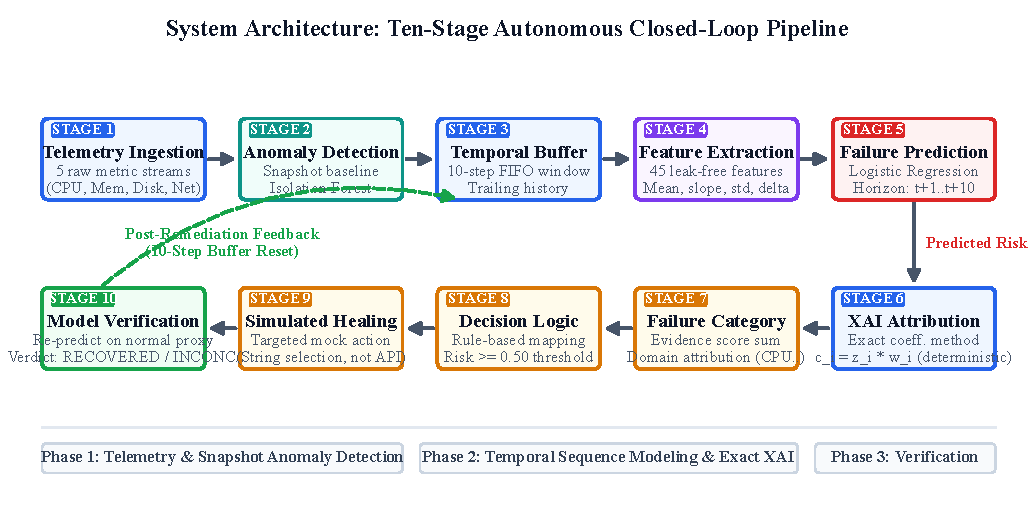
\includegraphics[width=0.92\columnwidth]{figures/fig1_system_architecture.pdf}
\caption{Explainable AI-driven cloud management system architecture (ten-stage pipeline).}
\label{fig:arch}
\end{figure}

The proposed platform comprises ten processing stages arranged as a sequential pipeline:
\begin{enumerate}
\item \textbf{Telemetry Ingestion:} Synthetic generation of multi-metric sequences across CPU, memory, disk, and network interfaces.
\item \textbf{Anomaly Detection:} Snapshot point-in-time detection using an unsupervised Isolation Forest model.
\item \textbf{Temporal Buffer Management:} 10-step sliding window aggregation to accumulate historical temporal context.
\item \textbf{Temporal Feature Extraction:} Derivation of 45 leak-free statistical and regression features across trailing windows.
\item \textbf{Failure Risk Prediction:} Sequence-level classification using Logistic Regression to predict future failure probability.
\item \textbf{XAI Attribution:} Deterministic feature contribution computation via exact model coefficients and normalized values.
\item \textbf{Likely Failure Category:} Evidence score aggregation across resource domains (CPU, Memory, Disk, Network).
\item \textbf{Autonomous Decision Logic:} Rule-based selection mapping inferred failure category to targeted remediation.
\item \textbf{Simulated Recovery:} Mock execution of recovery logic (string selection representing remediation action).
\item \textbf{Post-Recovery Verification:} Model-based re-evaluation of simulated recovered telemetry using the same trained classifier.
\end{enumerate}

\subsection{Temporal Feature Engineering}

A leak-free temporal feature set comprising 45 features is constructed from each 10-step trailing window. For each of the five raw metrics, nine features are computed: current value, 5-step mean, 10-step mean, 5-step delta, 10-step delta, 5-step slope (via linear regression), 10-step slope, 5-step standard deviation, and 10-step standard deviation. The feature extraction module strictly utilizes trailing observations, ensuring no access to future values (thereby preventing data leakage). A \texttt{StandardScaler} feature transformation is fitted exclusively on training rows and applied consistently during live inference.

\subsection{Predictive Modeling and Target Formulation}

Logistic Regression was selected for the integrated system with hyperparameters: regularisation strength $C = 1.0$, maximum iterations $\text{max\_iter} = 2000$, random seed 42, and balanced class weights (\texttt{class\_weight='balanced'}). The prediction target is strictly forward-looking and binary: a label of 1 denotes that an active failure occurs within the subsequent 10 future timesteps ($t+1 \le t' \le t+10$), strictly excluding the current observation at timestep $t$ to avoid target circularity, and 0 otherwise.

The model is trained at server initialisation on the Phase 3C seed-42 training split (4,920 rows from 120 sequences). The fitted scaler and model are used for all live inference. Logistic Regression is selected over Random Forest and Gradient Boosting not because it achieves the highest aggregate performance---all three achieve similar F1-scores and ROC-AUC values within measurement noise---but because its coefficient-based attribution is mathematically exact and requires no post-hoc approximation method.

\subsection{Explainable AI and Failure Categorization}

\subsubsection{Deterministic XAI Attribution}
For each live prediction, the linear contribution $c_i$ of temporal feature $i$ is computed deterministically as:
\begin{equation}
c_i = z_i \cdot w_i = \left(\frac{x_i - \mu_i}{\sigma_i}\right) w_i
\label{eq:attribution}
\end{equation}
where $z_i$ denotes the $z$-score standardized feature value derived using the training-set mean $\mu_i$ and standard deviation $\sigma_i$, and $w_i$ represents the learned Logistic Regression coefficient. The score $c_i$ quantifies the signed contribution of feature $i$ to the predicted failure log-odds. A positive value ($c_i > 0$) increases the estimated failure probability toward the high-risk threshold, whereas a negative value ($c_i < 0$) indicates evidence toward nominal operation. For operational transparency, the top five features ranked by absolute contribution $|c_i|$ are reported for each inference cycle.

\subsubsection{Likely Failure Category Inference}
Evidence scores across four primary resource domains (CPU, Memory, Disk, and Network) are obtained by summing the absolute attribution values of corresponding features:
\begin{equation}
E_r = \sum_{i \in \mathcal{F}_r} |c_i|
\label{eq:evidence}
\end{equation}
where $\mathcal{F}_r$ denotes the set of temporal features mapped to resource domain $r \in \{\text{CPU}, \text{Memory}, \text{Disk}, \text{Network}\}$. The domain with the highest aggregate evidence $\arg\max_r E_r$ is inferred as the likely failure category. This heuristic attribution summarizes model focus without asserting counterfactual causal proof.

\subsection{Decision and Simulated Self-Healing}

When predicted failure risk reaches the actionable threshold, the autonomous decision engine maps the inferred likely failure category to a simulated recovery procedure, as summarized in Table~\ref{tab:category_actions}.

\begin{table}[htbp]
\centering
\caption{LIKELY FAILURE CATEGORY TO SIMULATED RECOVERY ACTION MAPPING}
\label{tab:category_actions}
\begin{tabular}{ll}
\toprule
\textbf{Likely Failure Category} & \textbf{Simulated Recovery Action} \\
\midrule
CPU Spike & Terminate / throttle high-CPU processes \\
Memory Leak & Restart affected service / reclaim memory \\
Disk Exhaustion & Clear logs / archive data / expand storage \\
Network Degradation & Check / restart network service / reroute \\
Combined Failure & Controlled recovery sequence + operator alert \\
\bottomrule
\end{tabular}
\end{table}

\subsection{Post-Healing Verification Protocol}

When predicted failure risk reaches the HIGH or CRITICAL threshold ($\ge 0.50$):
\begin{enumerate}
\item Pre-healing risk (score, level, label) is recorded.
\item The decision engine selects a recovery action (simulated string selection, not executed via cloud API).
\item A 10-step synthetic stable normal telemetry sequence is generated as an algorithmic proxy for the recovered state.
\item The same trained Logistic Regression model evaluates this sequence.
\item Post-healing risk (score, level, label) is recorded.
\item Verification verdict determination:
\begin{itemize}
\item \textbf{RECOVERED}: Post-healing risk level is evaluated as LOW ($\le 0.25$).
\item \textbf{NOT\_RECOVERED}: Post-healing risk level remains HIGH or CRITICAL ($\ge 0.50$).
\item \textbf{INCONCLUSIVE}: Post-healing risk level is evaluated as MEDIUM ($0.25 < \text{risk} < 0.50$), indicating partial remediation without achieving full baseline stability.
\end{itemize}
\end{enumerate}

The temporal buffer is cleared after healing so that the subsequent polling cycle re-enters the \texttt{WARMING\_UP} state.

\section{Experimental Setup}

\subsection{Dataset Configuration and Splits}

The evaluation dataset encompasses eight distinct scenario profiles: two nominal baseline profiles (stable normal and variable normal) and six failure scenarios (CPU sudden failure, CPU gradual failure, gradual memory leak, gradual disk exhaustion, network degradation, and combined gradual failure). Across these eight scenarios, a total of 180 sequences were generated and partitioned into 120 training sequences (4,920 supervised rows), 30 validation sequences (1,230 supervised rows), and 30 test sequences (1,230 supervised rows). This yields exactly 7,380 supervised rows under a 10-step trailing window and 10-step prediction horizon censoring ($60 - 10 - 10 + 1 = 41$ rows per 60-step sequence), as summarized in Table~\ref{tab:splits}.

\begin{table}[htbp]
\centering
\caption{DATASET SPLITS AND SUPERVISED ROW COUNTS}
\label{tab:splits}
\begin{tabular}{lcc}
\toprule
\textbf{Split} & \textbf{Sequences} & \textbf{Supervised Rows} \\
\midrule
Training & 120 & 4,920 \\
Validation & 30 & 1,230 \\
Test & 30 & 1,230 \\
\textbf{Total} & \textbf{180} & \textbf{7,380} \\
\bottomrule
\end{tabular}
\end{table}

Sequence-level splitting ensures no temporal window from a test sequence is visible during training. Zero sequence overlap is verified by an automated audit.

\textbf{Positive label definition:} A timestep $t$ is labelled positive ($y_t = 1$) if an active failure is present in any of the next 10 future observations ($t+1 \le t' \le t+10$). The current observation at timestep $t$ is strictly excluded from the target calculation, ensuring that the model is trained exclusively on advance predictive indicators rather than instantaneous state detection. Positive samples constitute approximately 52\% of the dataset under this early-warning formulation.

\subsection{Anomaly Detection Evaluation (Phase 2)}

Isolation Forest is evaluated on snapshot telemetry. Baselines include a fixed-threshold classifier (alarm if any metric exceeds 80\%) evaluated on identical data.

\subsection{Temporal Predictive Evaluation (Phase 3)}

Five models are compared across five random seeds \{42, 123, 456, 789, 2026\}:
\begin{enumerate}
\item Majority-class baseline
\item Current-value threshold baseline
\item Logistic Regression ($C=1.0$, $\text{max\_iter}=2000$, \texttt{class\_weight='balanced'})
\item Random Forest ($n_{\text{estimators}}=100$, \texttt{class\_weight='balanced'})
\item Gradient Boosting ($n_{\text{estimators}}=100$)
\end{enumerate}

Performance metrics include accuracy, precision, recall, F1-score, Area Under the Receiver Operating Characteristic (ROC-AUC), and Precision-Recall Area Under Curve (PR-AUC).

\subsection{Early-Warning Horizon Evaluation}

Among test sequences containing labelled failure regions, the number of timesteps by which the model issues its first HIGH or CRITICAL prediction prior to the labelled failure onset is measured.

\subsection{Explainability Evaluation Protocol}

Representative XAI case studies are documented from test sequences across failure scenarios. For each case, the top five contributing features, their directions, and the evidence scores are recorded.

\section{Experimental Results and Analysis}

\subsection{Detection Performance (Phase 2)}
The baseline snapshot anomaly detection performance of Isolation Forest compared to the threshold baseline is shown in Table~\ref{tab:if_metrics}.

\begin{table}[htbp]
\centering
\caption{ANOMALY DETECTION: ISOLATION FOREST VS. THRESHOLD BASELINE}
\label{tab:if_metrics}
\resizebox{\columnwidth}{!}{
\begin{tabular}{lccccc}
\toprule
\textbf{Method} & \textbf{Accuracy} & \textbf{Precision} & \textbf{Recall} & \textbf{F1} & \textbf{FPR} \\
\midrule
Threshold Baseline & 0.903 & 1.000 & 0.435 & 0.606 & 0.000 \\
Isolation Forest & 0.910 & 0.704 & 0.826 & 0.760 & 0.073 \\
\bottomrule
\end{tabular}
}
\end{table}

The Isolation Forest achieves substantially higher recall than the threshold baseline (0.826 vs. 0.435), correctly identifying most failure events at the cost of a 7.3\% false positive rate. The threshold baseline produces zero false positives but misses 56.5\% of failures---particularly gradual-onset scenarios where no metric exceeds 80\% until late in the failure trajectory. Per-scenario detection analysis shows that CPU spike (F1 0.823), memory leak (F1 0.870), and network degradation (F1 1.000) are detected reliably. Disk gradual exhaustion achieves an F1-score of only 0.700 at snapshot level, reflecting the slow metric accumulation rate relative to the 80\% static threshold.

\subsection{Temporal Predictive Performance (Phase 3)}
The performance of the temporal predictive models aggregated over five independent random seeds is presented in Table~\ref{tab:model_comp} and illustrated in Fig.~\ref{fig:model_comp}.

\begin{table}[htbp]
\centering
\caption{TEMPORAL MODEL COMPARISON (5-SEED MEAN $\pm$ STD)}
\label{tab:model_comp}
\resizebox{\columnwidth}{!}{
\begin{tabular}{lccccc}
\toprule
\textbf{Model} & \textbf{F1} & \textbf{ROC-AUC} & \textbf{PR-AUC} & \textbf{Precision} & \textbf{Recall} \\
\midrule
Majority Baseline & 0.514 $\pm$ 0.259 & --- & --- & 0.380 $\pm$ 0.193 & 0.800 $\pm$ 0.400 \\
Threshold Baseline & 0.156 $\pm$ 0.054 & --- & --- & 0.997 $\pm$ 0.006 & 0.086 $\pm$ 0.031 \\
Logistic Regression & \textbf{0.692 $\pm$ 0.036} & 0.813 $\pm$ 0.021 & 0.840 $\pm$ 0.027 & 0.730 $\pm$ 0.049 & 0.661 $\pm$ 0.050 \\
Random Forest & \textbf{0.696 $\pm$ 0.021} & 0.819 $\pm$ 0.005 & 0.847 $\pm$ 0.017 & 0.805 $\pm$ 0.047 & 0.620 $\pm$ 0.057 \\
Gradient Boosting & \textbf{0.699 $\pm$ 0.030} & 0.826 $\pm$ 0.013 & 0.852 $\pm$ 0.025 & 0.747 $\pm$ 0.137 & 0.701 $\pm$ 0.127 \\
\bottomrule
\end{tabular}
}
\end{table}

\begin{figure}[htbp]
\centering
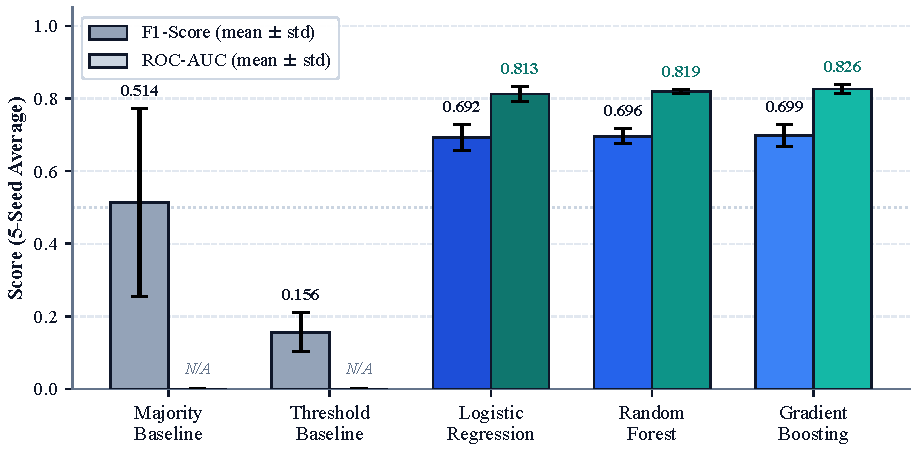
\includegraphics[width=0.92\columnwidth]{figures/fig4_model_comparison.pdf}
\caption{Temporal predictive model comparison across five random seeds (mean F1-score and ROC-AUC).}
\label{fig:model_comp}
\end{figure}

All three machine learning classifiers substantially outperform both baselines. The performance differences among Logistic Regression (LR), Random Forest (RF), and Gradient Boosting (GB) are small relative to within-seed variance. Gradient Boosting attains the highest mean F1-score (0.699) and ROC-AUC (0.826) but also exhibits the largest standard deviation in recall ($\pm$0.127). Logistic Regression demonstrates the most stable performance across seeds (F1-score standard deviation $\pm$0.036). At random seed 42 specifically, LR achieves F1-score 0.727 and ROC-AUC 0.830; RF achieves F1-score 0.718 and ROC-AUC 0.819; and GB achieves F1-score 0.725 and ROC-AUC 0.812.

\textbf{Threshold baseline analysis:} The current-value threshold baseline achieves high precision (0.997) but low recall (0.086)---it correctly identifies near-saturation events when a metric exceeds 80\%, but misses the vast majority of failure timesteps because gradual failures develop slowly below the threshold. This confirms that temporal feature-based prediction provides substantially better early-warning sensitivity.

\subsection{Per-Scenario Predictive Performance}
Table~\ref{tab:scenario_perf} reports the breakdown of classification performance across each evaluated failure scenario for Logistic Regression on the test split.

\begin{table}[htbp]
\centering
\caption{PER-SCENARIO PREDICTIVE PERFORMANCE (LOGISTIC REGRESSION, SEED 42, TEST SPLIT)}
\label{tab:scenario_perf}
\resizebox{\columnwidth}{!}{
\begin{tabular}{lcccccccc}
\toprule
\textbf{Scenario} & \textbf{Support} & \textbf{Prec} & \textbf{Recall} & \textbf{F1} & \textbf{TN} & \textbf{FP} & \textbf{FN} & \textbf{TP} \\
\midrule
Stable Normal & 205 & 0.00 & 0.00 & 0.00 & 132 & 73 & 0 & 0 \\
Variable Normal & 164 & 0.00 & 0.00 & 0.00 & 164 & 0 & 0 & 0 \\
CPU Sudden Failure & 41 & 0.529 & 0.529 & 0.529 & 16 & 8 & 8 & 9 \\
CPU Gradual Failure & 164 & 0.817 & 0.527 & 0.641 & 41 & 13 & 52 & 58 \\
Memory Gradual Leak & 41 & 1.000 & 0.649 & 0.787 & 4 & 0 & 13 & 24 \\
Disk Gradual Exhaustion & 246 & 0.952 & 0.791 & 0.864 & 12 & 9 & 47 & 178 \\
Network Degradation & 123 & 0.635 & 0.783 & 0.702 & 36 & 27 & 13 & 47 \\
Combined Gradual Failure & 246 & 0.820 & 0.755 & 0.786 & 56 & 27 & 40 & 123 \\
\bottomrule
\end{tabular}
}
\end{table}

Comparative inspection of the per-scenario classification outcomes reveals distinct operational behaviors:
\begin{itemize}
\item \textbf{Normal baseline profiles} produce zero true positives with moderate false positives (73 out of 205 for stable normal), reflecting the sensitivity orientation of balanced class weighting (\texttt{class\_weight='balanced'}).
\item \textbf{CPU sudden failure} yields the lowest F1-score (0.529), confirming the inherent boundary of temporal forecasting when abrupt step-function faults produce limited precursor trajectory signals prior to onset.
\item \textbf{Gradual failure modes} (gradual disk exhaustion, gradual memory leak, and combined failure) attain substantially higher F1-scores (0.786 to 0.864), demonstrating that rolling statistical features effectively capture accumulating degradation dynamics.
\item \textbf{Memory gradual leak} achieves perfect precision (1.000), confirming that all positive predictions on memory-leak sequences are valid, while recall (0.649) highlights the delay in accumulating sufficient temporal variation during early trajectory timesteps.
\end{itemize}

\subsection{Early-Warning Performance}
The advance warning horizon achieved across all evaluated failure sequences is detailed in Table~\ref{tab:early_warning}.

\begin{table}[htbp]
\centering
\caption{EARLY-WARNING LEAD TIME STATISTICS}
\label{tab:early_warning}
\begin{tabular}{lc}
\toprule
\textbf{Metric} & \textbf{Value} \\
\midrule
Failure sequences evaluated & 18 \\
Mean lead time (timesteps) & 18.06 \\
Median lead time & 16.0 \\
Minimum lead time & 4 \\
Maximum lead time & 33 \\
\bottomrule
\end{tabular}
\end{table}

The model issued at least one HIGH or CRITICAL prediction before the labelled failure onset across all 18 evaluated failure sequences. The mean lead time of 18.06 timesteps represents substantial advance warning. The minimum lead time of 4 timesteps occurred on sudden-failure scenarios, which is consistent with the lower predictive sensitivity observed on abrupt faults.

\subsection{XAI Attribution Case Studies}
Table~\ref{tab:xai_cases} summarizes representative XAI attribution case studies, with corresponding feature contributions visualized in Fig.~\ref{fig:xai}.

\begin{table}[htbp]
\centering
\caption{REPRESENTATIVE XAI ATTRIBUTION CASE STUDIES}
\label{tab:xai_cases}
\resizebox{\columnwidth}{!}{
\begin{tabular}{lllllll}
\toprule
\textbf{Case} & \textbf{Scenario} & \textbf{Risk} & \textbf{Top Feature} & \textbf{Contrib} & \textbf{Dir} & \textbf{Likely Cat} \\
\midrule
test\_1 & Disk Gradual & 0.591 & Mem 10-step avg & -0.999 & $\downarrow$ & Combined \\
test\_4 & Combined Gradual & 0.537 & CPU 10-step var & -0.422 & $\downarrow$ & Combined \\
test\_6 & Network Degrade & 0.534 & Mem 10-step var & +0.416 & $\uparrow$ & Combined \\
test\_15 & CPU Sudden & 0.686 & Mem 10-step avg & +0.917 & $\uparrow$ & Memory Leak \\
\bottomrule
\end{tabular}
}
\end{table}

\begin{figure}[htbp]
\centering
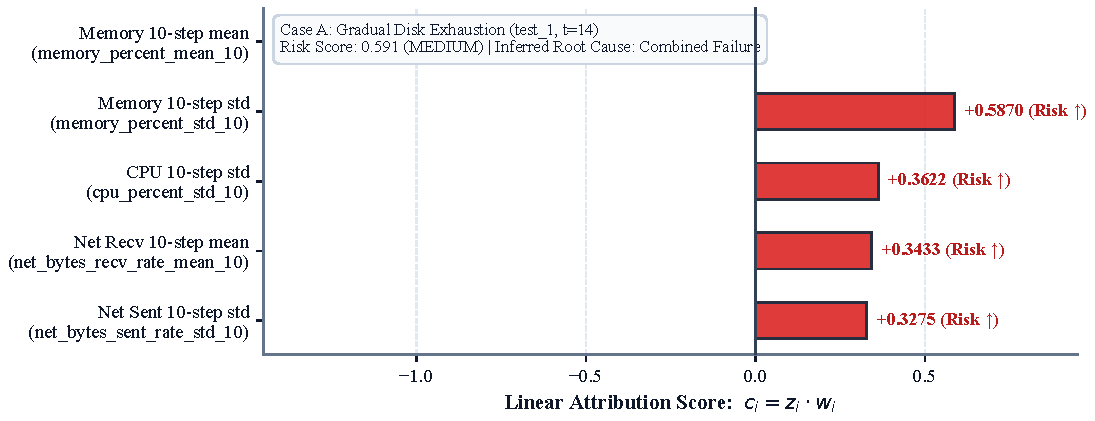
\includegraphics[width=0.92\columnwidth]{figures/fig6_xai_contributions.pdf}
\caption{Deterministic XAI feature contributions for a representative evaluation case (gradual disk exhaustion).}
\label{fig:xai}
\end{figure}

The XAI attribution analysis reveals that variability features (standard deviation) and trend features (slope) frequently dominate feature contributions in gradual failure scenarios. This reflects that incipient failures increase temporal variation and trend steepness before raw metric magnitudes cross alarm thresholds. In several cases, rolling mean memory features exhibit negative contributions; here, the model interprets elevated average memory as evidence against a specific isolated failure label, which is consistent with multi-resource patterns learned from combined failure sequences.

\subsection{Integrated Recovery Verification}

The integrated system was evaluated across all six failure scenarios. For the network degradation scenario, the simulated verification sequence and resulting risk transition are reported in Table~\ref{tab:verification} and depicted in Fig.~\ref{fig:verification}:

\begin{table}[htbp]
\centering
\caption{POST-RECOVERY VERIFICATION EVALUATION (NETWORK DEGRADATION)}
\label{tab:verification}
\begin{tabular}{ll}
\toprule
\textbf{Stage} & \textbf{Value} \\
\midrule
Pre-healing risk & CRITICAL (0.884) \\
Simulated recovery & Controlled recovery sequence + alert \\
Post-healing risk & MEDIUM (0.447) \\
Verification verdict & INCONCLUSIVE \\
\bottomrule
\end{tabular}
\end{table}

\begin{figure}[htbp]
\centering
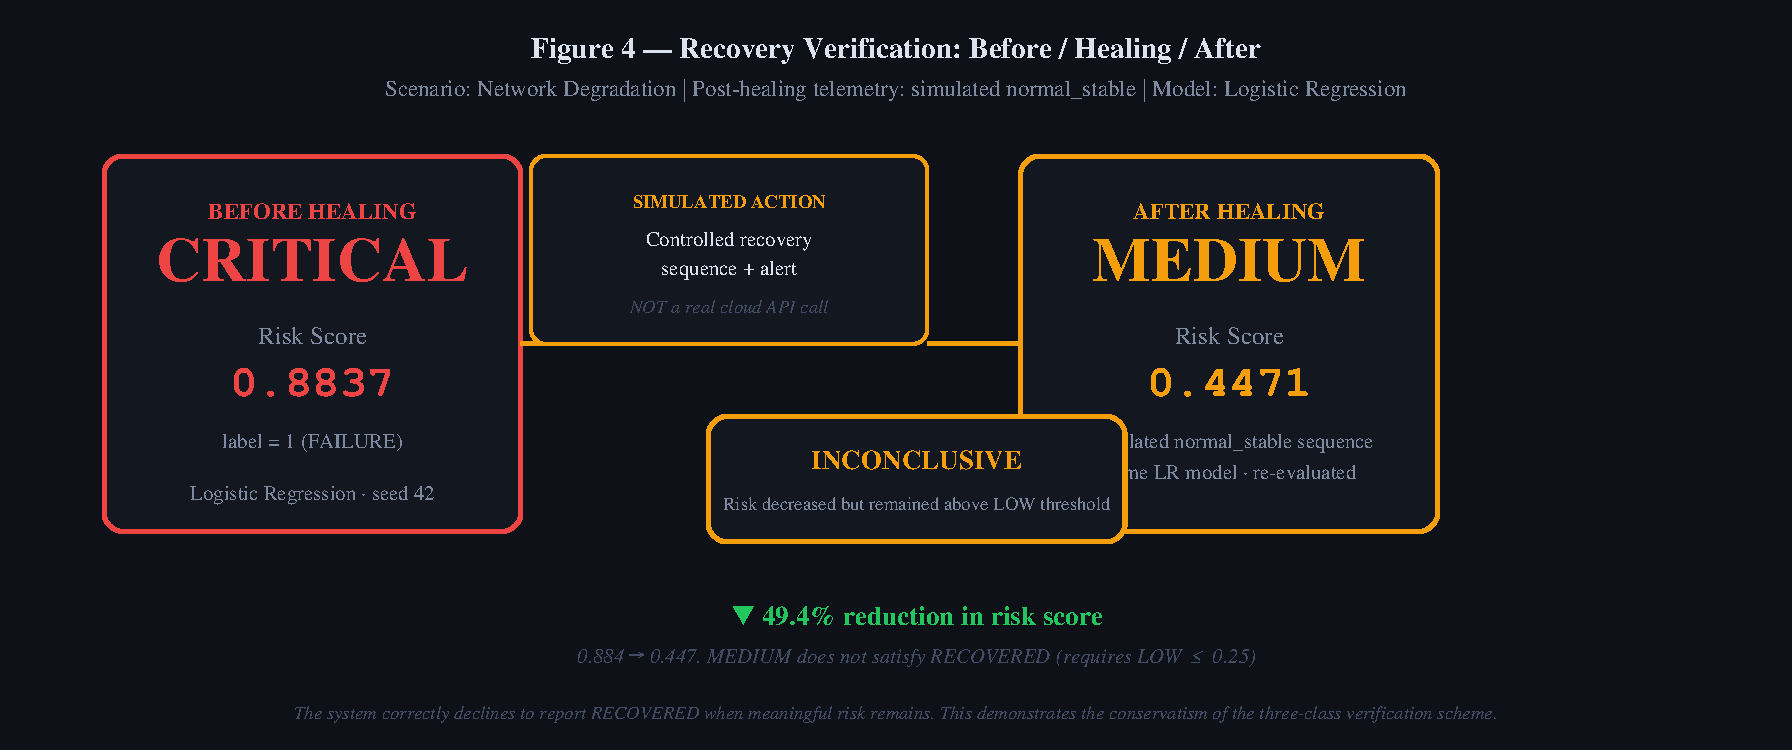
\includegraphics[width=0.92\columnwidth]{figures/fig7_verification.pdf}
\caption{Closed-loop post-recovery verification flow for the network degradation scenario.}
\label{fig:verification}
\end{figure}

In this evaluation, the estimated failure risk decreased substantially from pre-healing CRITICAL (0.884) to post-healing MEDIUM (0.447), but remained above the LOW threshold ($\le 0.25$), resulting in an INCONCLUSIVE verification verdict. This outcome represents an expected and operationally honest evaluation: the verification engine evaluates the post-remediation state against a simulated synthetic normal stream, which may still contain residual variance that keeps the score in the medium-risk band. Remediation actions in this research prototype are simulated string selections dispatched by the rule-based engine rather than destructive cloud orchestration API calls. Similarly, post-healing telemetry is synthetically generated normal data serving as an algorithmic verification proxy rather than a physical infrastructure recovery. By returning INCONCLUSIVE rather than overstating success, the system demonstrates necessary operational conservatism.

\section{Discussion}

\subsection{Temporal Features vs. Threshold Detection}

The results confirm that temporal rolling features substantially improve early-warning performance compared with snapshot threshold monitoring. The threshold baseline achieves a mean recall of only 8.6\% across seeds because gradual failures accumulate below any fixed threshold until late in the sequence. Logistic Regression with temporal features achieves a mean recall of 66.1\% with an advance lead time averaging 18.06 timesteps. This demonstrates the operational advantage of temporal sequence modeling over instantaneous point-in-time checks.

\subsection{Model Selection Trade-offs}

Random Forest and Gradient Boosting achieve marginally higher mean F1-scores and ROC-AUC values than Logistic Regression, but the differences remain within random seed variance. The decision to integrate Logistic Regression is justified by interpretability: its coefficient-based attribution is mathematically exact, computationally lightweight, and requires no sampling approximations such as SHAP or LIME. This represents a deliberate, principled system-design trade-off.

\subsection{XAI for Operational Context}

The coefficient attribution results indicate that variability (standard deviation) and trend (slope) features are the primary predictive drivers for gradual failure scenarios. This offers actionable diagnostic clarity: a systems operator informed that the ``CPU 5-step slope is the strongest positive contributor'' can inspect the corresponding CPU trend chart and verify the alert independently without relying on an unverified black-box approximation.

\subsection{Root-Cause Inference Limitations}

The heuristic for likely failure categories reliably identifies the primary faulty resource for gradual single-resource scenarios. However, it exhibits limitations on sudden step-function failures (where temporal variation has not yet accumulated) and on combined failure modes (where attribution is distributed across multiple resource types). These failure modes are documented and consistent with the inherent constraints of sequence modeling. The system explicitly does not claim mechanistic or counterfactual causal discovery.

\subsection{Post-Recovery Verification Conservatism}

The INCONCLUSIVE verdict for the network degradation scenario represents an honest, conservative outcome. An operational platform that claimed RECOVERED whenever failure risk decreased by any non-zero margin would introduce hazardous false confidence. The three-state verification logic (RECOVERED, NOT\_RECOVERED, INCONCLUSIVE) enforces an essential standard of operational caution, preventing partial mitigations from being misclassified as complete recoveries.

\section{System Limitations and Threats to Validity}

\begin{enumerate}
\item \textbf{Synthetic telemetry:} All data is generated by parameterised scenario profiles rather than real production systems. Generalisation to physical multi-tenant cloud infrastructure remains unvalidated.
\item \textbf{Simulated recovery:} Remediation actions are logged string selections dispatched by rule-based logic, not executable hypervisor or cloud provider API calls. No real cloud resource reallocation occurs.
\item \textbf{Sudden failure detection bounds:} Abrupt step-function faults produce lower predictive sensitivity (F1 0.529) due to the absence of precursor trend signals in historical windows.
\item \textbf{Root-cause inference is not causal proof:} Evidence scores aggregate XAI contributions across resource domains; this heuristic mapping reflects model focus rather than formal counterfactual causal mechanisms.
\item \textbf{Post-healing telemetry is synthetic:} The verification verdict reflects model behaviour on simulated normal telemetry streams rather than physical platform recovery.
\item \textbf{Prototype model training at initialisation:} The research prototype fits the model at server startup, which is appropriate for evaluation and reproducibility but requires dedicated model registries in production.
\item \textbf{No real-world validation:} Benchmarking against production infrastructure traces (e.g., Alibaba Cluster, Google Cluster, or Microsoft Azure trace datasets) represents essential future work.
\end{enumerate}

\section{Conclusion and Future Work}

This paper presented an integrated, explainable AI-driven cloud management prototype that connects telemetry ingestion, Isolation Forest anomaly detection, temporal feature extraction, comparative predictive modeling, deterministic coefficient attribution, failure-category inference, autonomous decision logic, simulated recovery, and post-recovery model-based verification within a single evaluated system.

The key experimental findings are:
\begin{itemize}
\item Isolation Forest achieves an F1-score of 0.760 on snapshot anomaly detection.
\item Temporal Logistic Regression achieves mean F1-score 0.692 and ROC-AUC 0.813 across five seeds, substantially outperforming threshold-based monitoring (F1 0.156).
\item The model provides early-warning predictions with a mean lead time of 18.06 timesteps before labelled failure onset.
\item Deterministic coefficient attribution identifies variability and slope features as the strongest predictive drivers for gradual failure scenarios.
\item The post-recovery verification mechanism conservatively returns an INCONCLUSIVE verdict when recovery is partial, thereby preventing false claims of successful remediation.
\end{itemize}

Future work will address the validation of these methods on real cloud infrastructure trace datasets, the replacement of simulated recovery with real orchestration API integration, the evaluation of multi-model ensemble attribution methods, and rigorous comparisons with deep learning temporal methods (e.g., LSTM and transformer networks) under identical experimental protocols.

\newpage
\section*{Acknowledgment}
The author expresses sincere gratitude to project guide Mrs.~S.~Shirly, Assistant Professor, Department of Computer Science and Engineering, Karunya Institute of Technology and Science, for her invaluable supervision, guidance, and constructive feedback throughout this research. In compliance with IEEE author guidelines, the author acknowledges the use of AI tools for assistance with manuscript language refinement and formatting; all technical concepts, experimental analyses, and conclusions were independently conducted, verified, and approved by the author.

\balance
\interlinepenalty=500
\bibliographystyle{IEEEtran}
\bibliography{references}

\end{document}
